%%%%%%%%%%%%%%%%%%%%%%%%%%%%%%%%%%%%%%%%%%%%%%%%%%%%%%%%%%%%%%%%%%%
%%% Documento LaTeX 																						%%%
%%%%%%%%%%%%%%%%%%%%%%%%%%%%%%%%%%%%%%%%%%%%%%%%%%%%%%%%%%%%%%%%%%%
% T�tulo:		Cap�tulo 2
% Autor:  	Ignacio Moreno Doblas
% Fecha:  	2014-02-01
% Versi�n:	0.5.0
%%%%%%%%%%%%%%%%%%%%%%%%%%%%%%%%%%%%%%%%%%%%%%%%%%%%%%%%%%%%%%%%%%%
\chapterbegin{Resultados}
\label{chp:Resultados}

\section{Reconstruccion}

\newpage
\section{Clasificaci�n}




\begin{figure}[!hb]
\centering
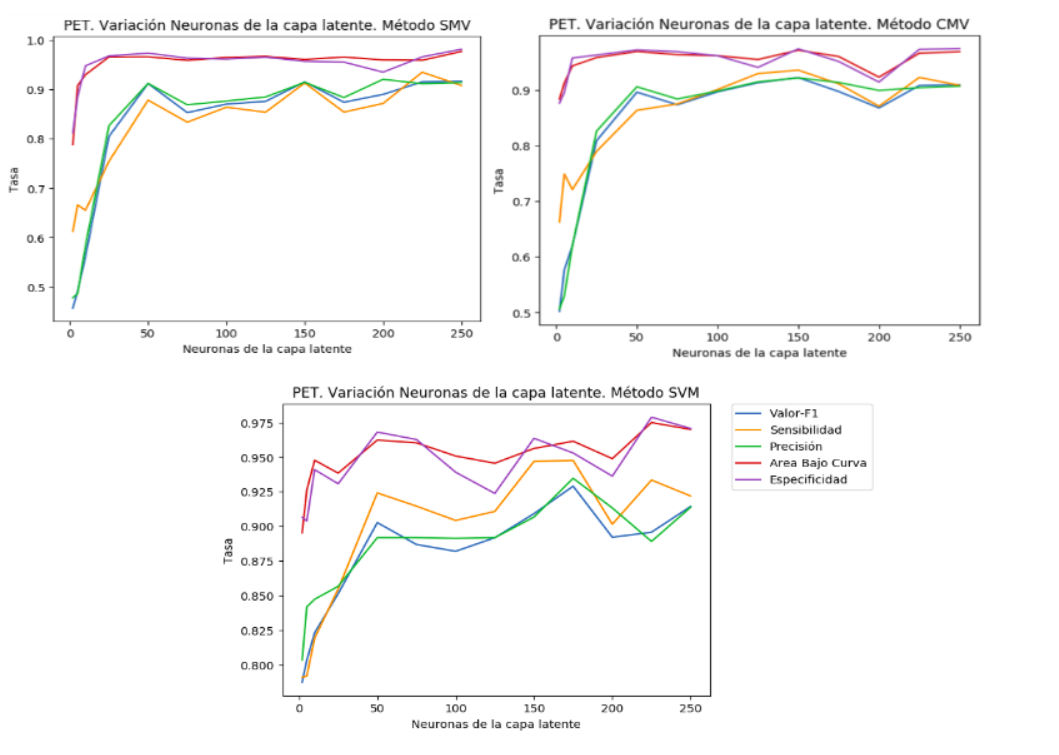
\includegraphics[scale=0.40]{images/SweepLatentLayerPET.png}
\caption{Resultados de clasificaci�n sobre las im�genes PET aplicando las tres t�cnicas de evaluacion conjunta de resultados. (Izquierda) Voto por Mayor�a Simple. (Centro) M�quina de Vectores de Soporte. (Derecha) Voto por Mayor�a Complejo.}
\label{fig:curva_roc}
\end{figure}


\begin{figure}[!hb]
\centering
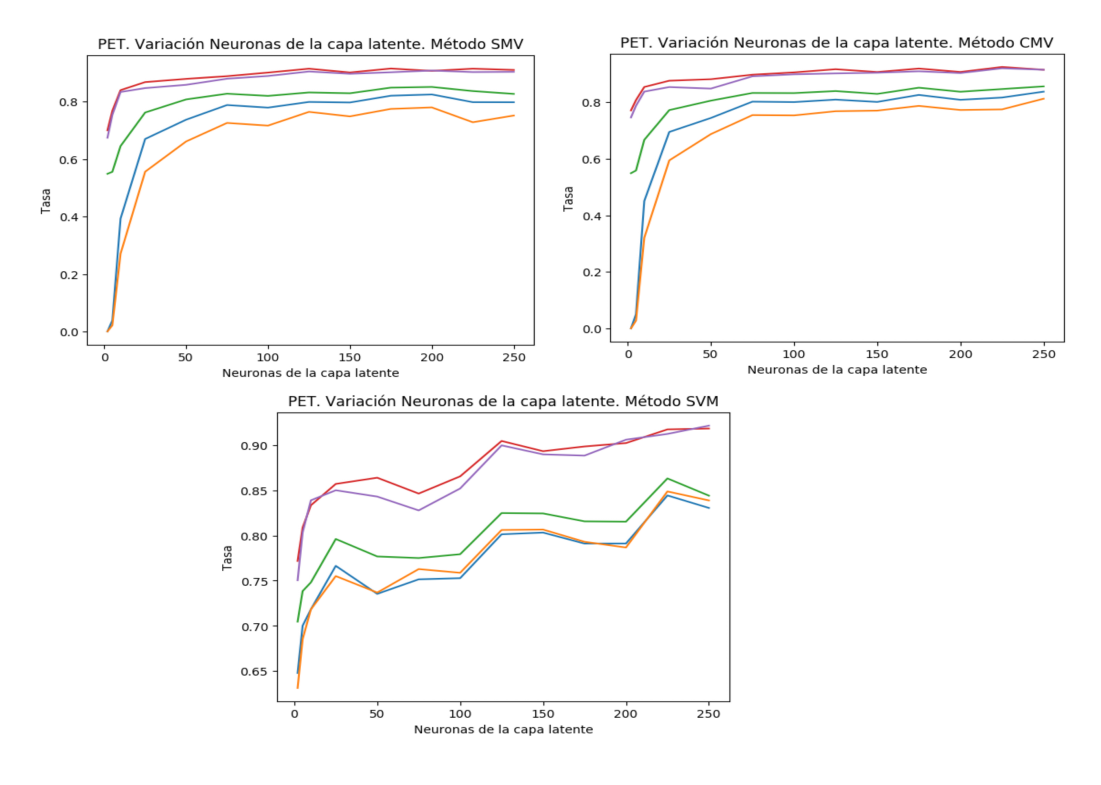
\includegraphics[scale=0.40]{images/MRI_VAE_LatentLayer.png}
\caption{Resultados de clasificaci�n sobre las im�genes MRI aplicando las tres t�cnicas de evaluacion conjunta de resultados. (Izquierda) Voto por Mayor�a Simple. (Centro) M�quina de Vectores de Soporte. (Derecha) Voto por Mayor�a Complejo.}
\label{fig:curva_roc}
\end{figure}



%\minitoc
\chapterend{}